\documentclass{article}
\usepackage{amsmath}
\usepackage{tikz}
\usetikzlibrary{arrows.meta}

\begin{document}

\title{Análisis de Influencia en una Red Social con Tipos de Interacción}
\author{}
\date{}
\maketitle

\section*{Problema: Análisis de Influencia en una Red Social con Tipos de Interacción}

Un investigador de redes sociales está estudiando una red de seis usuarios en una plataforma social (A, B, C, D, E y F). Cada usuario tiene distintos tipos de interacciones con otros usuarios de la red, como menciones, retuits y comentarios. La influencia de cada usuario sobre otro varía según la frecuencia y el tipo de interacción.

La red se representa mediante una \textbf{matriz de influencia ponderada} \( A \), donde cada entrada \( A_{ij} \) indica la fuerza de la influencia del usuario \( j \) sobre el usuario \( i \). Esta matriz de influencia está dada por:

\[
A = \begin{bmatrix} 
0 & 0.5 & 0.3 & 0 & 0 & 0.4 \\ 
0.2 & 0 & 0.4 & 0.1 & 0.3 & 0 \\ 
0.6 & 0.3 & 0 & 0 & 0.2 & 0.5 \\ 
0 & 0 & 0.5 & 0 & 0.6 & 0.4 \\ 
0.4 & 0.2 & 0 & 0.3 & 0 & 0.1 \\ 
0.3 & 0 & 0.5 & 0 & 0.2 & 0 
\end{bmatrix}
\]

Aquí:
- Cada valor en la matriz \( A_{ij} \) indica cuánto influye el usuario \( j \) sobre el usuario \( i \) en el contexto de interacciones en la plataforma.
- Los valores más altos indican una influencia mayor entre los usuarios.

\section*{Objetivo}

El objetivo es determinar la \textbf{influencia a largo plazo} de cada usuario en la red. Este análisis puede ayudar a entender qué usuarios tienen el mayor poder de influencia en la red y cómo se distribuye esta influencia.

\section*{Preguntas}

\begin{enumerate}
    \item (a) Encuentre los autovalores de la matriz \( A \) resolviendo el polinomio característico \(\text{det}(A - \lambda I) = 0\).

    \item (b) Determine el autovalor dominante (el autovalor con el mayor valor absoluto) y su autovector correspondiente, que indicará la influencia relativa de cada usuario en la red.

    \item (c) Normalice el autovector dominante de forma que la suma de sus entradas sea igual a 1. Esto representa la \textbf{distribución de influencia a largo plazo} de cada usuario.

    \item (d) Analice los resultados:
    \begin{itemize}
        \item ¿Cuál usuario tiene la mayor influencia en la red a largo plazo?
        \item ¿Cómo se distribuye la influencia en la red a largo plazo?
    \end{itemize}

    \item (e) Simulación con Interacción Asimétrica: Suponga que se añade una interacción unilateral donde el usuario \( E \) tiene una fuerte influencia adicional sobre \( F \) con un valor de 0.7. Actualice la matriz \( A \) y repita el análisis.
\end{enumerate}


\section*{Red Social Gráfica}

\begin{center}
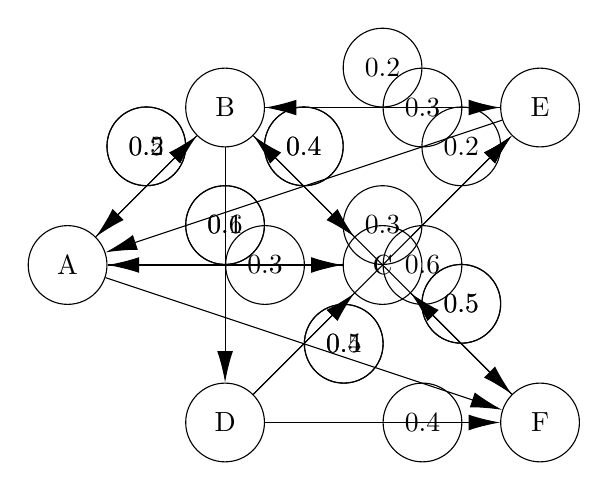
\begin{tikzpicture}[
  every node/.style={circle, draw, minimum size=1cm}, 
  every edge/.style={draw, -{Latex[width=2mm,length=4mm]}}]
  
  \node (A) at (0, 0) {A};
  \node (B) at (2, 2) {B};
  \node (C) at (4, 0) {C};
  \node (D) at (2, -2) {D};
  \node (E) at (6, 2) {E};
  \node (F) at (6, -2) {F};

  \path (A) edge node[above] {0.5} (B);
  \path (A) edge node[right] {0.3} (C);
  \path (A) edge node[right] {0.4} (F);
  
  \path (B) edge node[above] {0.2} (A);
  \path (B) edge node[above] {0.4} (C);
  \path (B) edge node[above] {0.1} (D);
  \path (B) edge node[right] {0.3} (E);
  
  \path (C) edge node[above] {0.6} (A);
  \path (C) edge node[above] {0.2} (E);
  \path (C) edge node[above] {0.5} (F);
  
  \path (D) edge node[right] {0.5} (C);
  \path (D) edge node[right] {0.6} (E);
  \path (D) edge node[right] {0.4} (F);
  
  \path (E) edge node[above] {0.4} (A);
  \path (E) edge node[above] {0.2} (B);
  
  \path (F) edge node[above] {0.3} (B);
  \path (F) edge node[above] {0.5} (C);
  
\end{tikzpicture}
\end{center}

Cada nodo en el grafo representa un usuario (A, B, C, D, E, F), y cada flecha muestra la dirección y fuerza de la influencia entre usuarios. El grosor de cada flecha representa la magnitud de la influencia según el valor en la matriz \( A \).

\end{document}
